% !TEX root = ../../main.tex

\section{Résultats numériques}

Dans cette section on s'intéresse à des résultats numériques pour la résolution du modèle VHL par les méthodes présentées précédemment. Conformément à~\cite{Holderied:2020}, nous considérons la conidition initiale suivante :
$$
  f_h(t=0,z,\vb{v}) = \frac{\rho_h}{(2\pi)^{3/2}\bar{v}_{\|}\bar{v}_\perp^2}\exp( - \frac{v_z^2}{2\bar{v}_{\|}^2} - \frac{\left( v_x^2 + v_y^2 \right)^2}{2\bar{v}_\perp^2} )
$$
avec $z\in[0,\frac{2\pi}{k}]$, $k=2$, $\bar{v}_{\|}=0.2$, $\bar{v}_\perp=0.6$, $\rho_h=0.2$ et $B_x(t=0,z)=\epsilon\sin(kz)$. Les autres inconnues du système $(j_{c,x},j_{c,y},B_y,E_x,E_y)$ sont initialisées à zéro. Le domaine en vitesse est restreint à $\vb{v}\in[-3.6,3.6]\times[-3.6,3.6]\times[-2.4,2.4]$ et on note $N_z$, $N_{v_x}$, $N_{v_y}$, $N_{v_z}$ le nombre de points de discrétisation dans chaque direction. Dans chacune des simulations, on s'intéresse à l'évolution temporelle des énergies suivantes :
\begin{description}
  \item[Énergie magnétique : ] $$\mathcal{H}_B(t) = \frac{1}{2}\int \left( B_x^2(t,z) + B_y^2(t,z) \right)\dd{z}$$
  \item[Énergie électrique : ] $$\mathcal{H}_E(t) = \frac{1}{2}\int \left( E_x^2(t,z) + E_y^2(t,z) \right)\dd{z}$$
  \item[Énergie cinétique des particules froides : ] $$\mathcal{H}_c(t) = \frac{1}{2\Omega_{pe}^2}\int \left( j_{c,x}^2(t,z) + j_{c,y}^2(t,z) \right)\dd{z}$$
  \item[Énergie cinétique des particules chaudes :  ] $$\mathcal{H}_h(t) = \frac{1}{2}\iint |\vb{v}|^2 f_h(t,z,\vb{v}) \dd{\vb{v}}\dd{z}$$
\end{description}
dont la somme, l'énergie totale, est préservée au cours du temps :
$$
  \dv{\mathcal{H}}{t} = \dv{\mathcal{H}_B+\mathcal{H}_E+\mathcal{H}_c+\mathcal{H}_h}{t} = 0.
$$


%%%%%%%%%%%%%%%%%%%%%%%%%%%%%%%%%%%%%%%%%%%%%%%%%%%%%%%%%%%%%%%%%%%%%

\subsection{Comparaison des solveurs à pas de temps constant}
% -------------------------------------------------------------------

\begin{figure}[h]
  \centering
  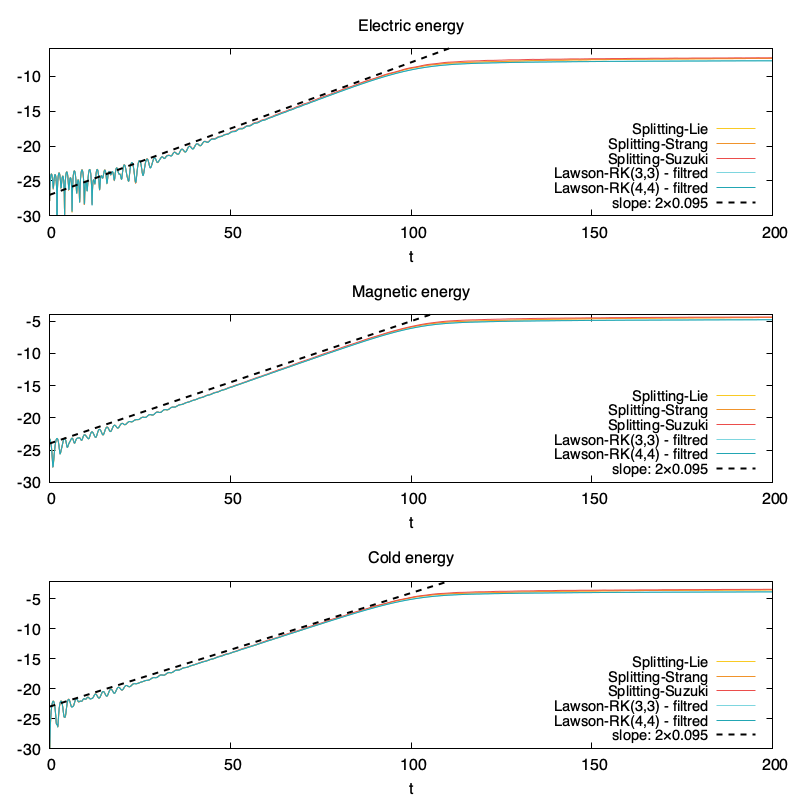
\includegraphics[width=0.9\textwidth]{\localPath/figures/energy_a_vmhl.png}
  \caption{Time evolution of the electric energy, the magnetic energy and the energy of cold particles defined in \eqref{energies}, in semi-$\log$ scale for Strang and Lawson-RK(3, 3). $\Delta t = 0.05, N_x=27, N_{v_x}=32, N_{v_y}=32, N_{v_z}=41$.}
  \label{fig:energies4d}
\end{figure}

\begin{figure}[h]
  \centering
  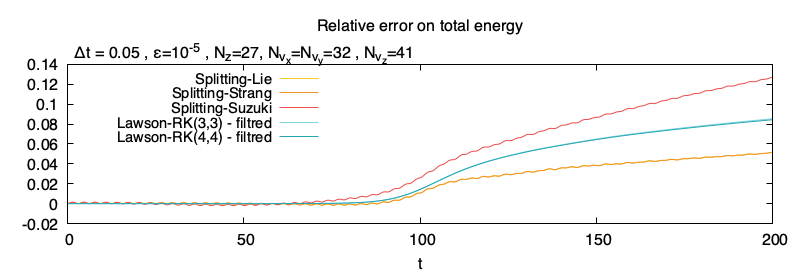
\includegraphics[width=0.9\textwidth]{\localPath/figures/H_a_vmhl.png}
  \caption{Time evolution of the total energy for Strang and Lawson-RK(3, 3). $\Delta t = 0.05, N_x=27, N_{v_x}=32, N_{v_y}=32, N_{v_z}=41$.}
  \label{fig:energy_tot4d}
\end{figure}

\begin{figure}[h]
  \centering
  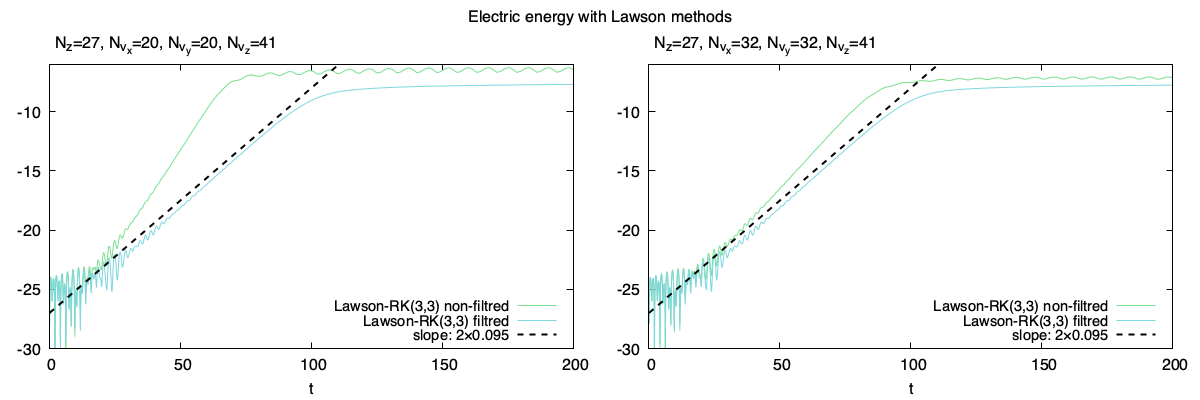
\includegraphics[width=0.9\textwidth]{\localPath/figures/ee_filtrage_vmhl.png}
  \caption{Time evolution of the electric energy for the filtered and unfiltered versions of Lawson-RK(3, 3). Left: $\Delta t = 0.05, N_x=27, N_{v_x}=20, N_{v_y}=20, N_{v_z}=41$. Right: $\Delta t = 0.05, N_x=27, N_{v_x}=32, N_{v_y}=32, N_{v_z}=41$}
  \label{fig:compar_ee4d}
\end{figure}


%%%%%%%%%%%%%%%%%%%%%%%%%%%%%%%%%%%%%%%%%%%%%%%%%%%%%%%%%%%%%%%%%%%%%

\subsection{Étude à pas de temps adaptatif}
% -------------------------------------------------------------------

\begin{figure}[h]
  \centering
  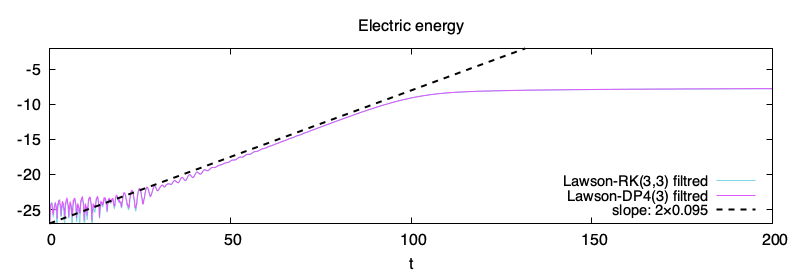
\includegraphics[width=0.9\textwidth]{\localPath/figures/energy_dp43_vmhl.png}
  \caption{Time evolution of the electric energy defined in \eqref{energies}, in semi-$\log$ scale for Lawson-RK(3, 3) ($\Delta t=0.05$) and Lawson-DP4(3). $N_x=27, N_{v_x}=32, N_{v_y}=32, N_{v_z}=41$.}
  \label{fig:energieselecdp43}
\end{figure}

\begin{figure}[h]
  \centering
  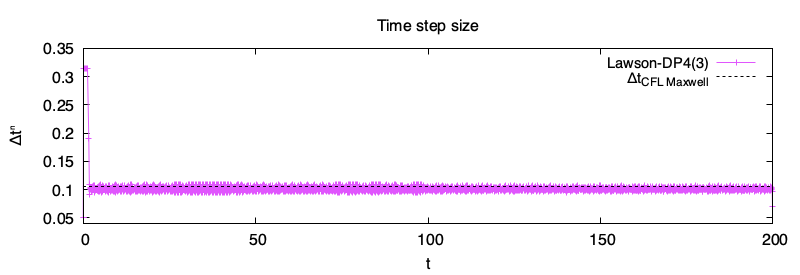
\includegraphics[width=0.9\textwidth]{\localPath/figures/dt_size_vmhl.png}
  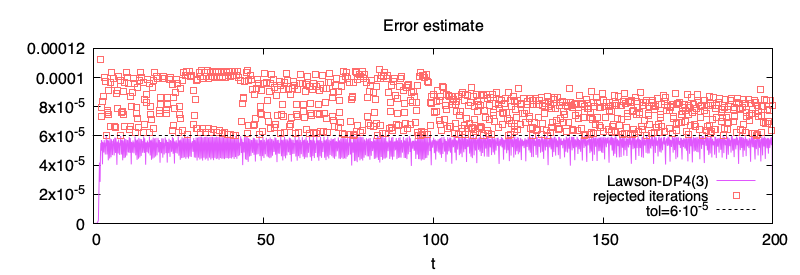
\includegraphics[width=0.9\textwidth]{\localPath/figures/L_vmhl.png}
  \caption{Time evolution of the time step (top) and the local error (bottom) for Lawson-DP4(3). $N_x=27, N_{v_x}=32, N_{v_y}=32, N_{v_z}=41$.}
  \label{fig:dtanderrordp43}
\end{figure}

